%\documentclass{article}
%
%\usepackage[pdftex,active,tightpage]{preview}
%\usepackage{tikz}
%\usepackage{pgfplots}
%\usetikzlibrary{plotmarks}
%
%\begin{document}
%\begin{preview}

	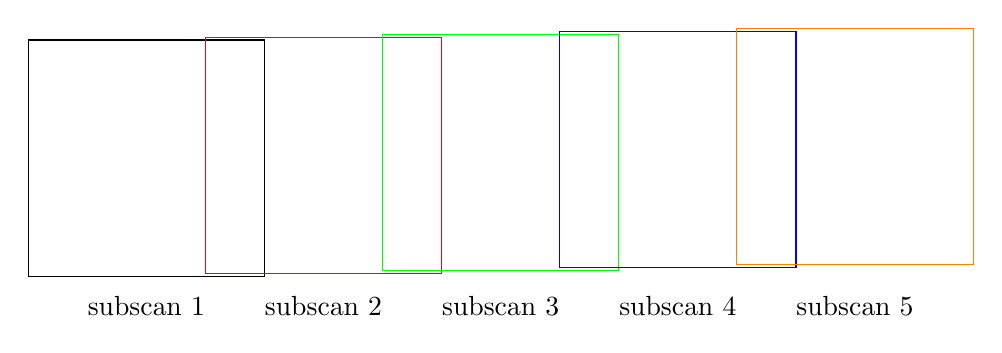
\begin{tikzpicture}[scale=.75]
		\foreach \x/\color in {0/black,
							1/red,
                         	2/green,
                         	3/blue,
                         	4/orange}
    	\draw[color=\color] (3*\x,.05*\x) rectangle (3*\x+4,.05*\x+4);
    	\foreach \x/\name in {0/1,1/2,2/3,3/4,4/5}
   		\draw (3*\x+2,-.5) node [color=black] {subscan \name};
	\end{tikzpicture}
%
%\end{preview}
%\end{document}